\documentclass[11pt]{article}
\usepackage[a4paper,margin=1in]{geometry}
\usepackage{booktabs}
\usepackage{amsmath}
\usepackage{array}
\usepackage{xcolor}
\usepackage{longtable}
\usepackage{pgfplots}
\pgfplotsset{compat=1.18}
\usepgfplotslibrary{groupplots}
\usepackage[hidelinks]{hyperref}
\usepackage{caption}

\definecolor{cArm}{HTML}{4677C8}
\definecolor{cRv}{HTML}{B5651D}
\definecolor{cBase}{HTML}{999999}

\newcommand{\code}[1]{\texttt{#1}}
\newcommand{\ms}{\texttt{\_\_mulsf3}}
\newcommand{\as}{\texttt{\_\_addsf3}}
\newcommand{\ds}{\texttt{\_\_divsf3}}

\title{\textbf{AVR-XPU Feasibility: Workload Characterization, Roofline,\\ and Baseline Comparison}\\[2pt]
\large An eXtensible AVR-derived datapath for edge flight-control / DSP / inference}
\author{Ashutosh Vishwakarma}
\date{June 2026}

\begin{document}
\maketitle

\begin{abstract}
This report presents the measured evidence for the AVR-XPU feasibility study, covering the first three
gates of the plan: \textbf{(\S1)} workload characterization, \textbf{(\S2)} a roofline / headroom model,
and \textbf{(\S3)} a baseline comparison against FPU-equipped ARM and RISC-V. Thirteen representative
flight-control, DSP, and quantized-inference kernels were run cycle-by-cycle on an instrumented gem5 AVR
model, each validated bit-for-bit against a host reference. The central findings are: (i) on the baseline
8-bit AVR core every fp kernel is \emph{compute-bound by software floating point}---58--98\,\% of cycles
are spent in softfloat helper routines, at $\sim$100--170 cycles per fp operation; (ii) the kernels have
\emph{low arithmetic intensity} (0.08--0.61 ops/byte), so once arithmetic is moved into hardware they
become \emph{memory-bound}---a hardware fp/MAC datapath yields $\approx$6--16$\times$ but \emph{wide SIMD
does not help}; and (iii) an FPU-equipped ARM/RISC-V core executes the same fp kernels in
\textbf{17--76$\times$ fewer instructions} than AVR softfloat, so AVR-XPU cannot win on raw throughput and
must instead target energy/area for a stripped, domain-specific datapath. All results are reproducible
from the public repositories and the logged per-run data.
\end{abstract}

\section{Introduction}
\textbf{AVR-XPU} is a proposed eXtensible, AVR-derived SIMD/MAC datapath for offloading the compute-heavy
kernels of a drone flight stack---extended Kalman filtering (sensor fusion), DSP, and lightweight
quantized inference---validated in gem5 with an FPGA proof-of-concept as the eventual target. Before
committing to RTL, the feasibility plan demands cheap, falsifiable evidence: \emph{what do the workloads
actually use, is the idea even compute-bound, and what does it have to beat?} This report answers those
three questions with measured data, not intuition.

The study is built on a custom gem5 AVR model (functionally and cycle validated against a real
ATmega328P). For this work the model was hardened and instrumented (\S\ref{sec:method}), and a
deterministic measurement harness was built so every run is reproducible and bit-exact-validated.

\section{Methodology}\label{sec:method}

\paragraph{Platform and ``eXtensible'' gem5 changes.}
Kernels run in gem5 syscall-emulation mode on the AVR model. Four changes were made to the model during
this study, each driven by a measurement need:
\begin{itemize}
  \item \textbf{Hard-halt on unknown opcodes.} The port previously \emph{skipped} undecoded instructions
  (silently corrupting results); it now halts and prints the offending opcode + PC. This made ISA gaps
  visible rather than masquerading as ``successful'' runs.
  \item \textbf{ELPM + RAMPZ.} Implementing \code{ELPM} (and aliasing the \code{RAMPZ} I/O register)
  unblocked workloads whose working set forces a $\geq$8\,KB-SRAM (hence $>$64\,KB-flash) device, whose
  C runtime copies \code{.data} with \code{ELPM}.
  \item \textbf{Op-mix instrumentation.} The CPU now emits, at exit, per-mnemonic instruction and cycle
  histograms, a per-function (PC$\rightarrow$symbol) instruction and cycle histogram, and a per-function
  \emph{call-count} histogram. These are the raw material for \S1--\S3.
\end{itemize}
The model + ISA work live in a gem5 fork (\href{https://github.com/ragnar-vallhala/gem5}{ragnar-vallhala/gem5},
branch \code{btp}); the harness and all data live in
\href{https://github.com/ragnar-vallhala/AVR-XPU}{ragnar-vallhala/AVR-XPU}.

\paragraph{Harness and validation oracle.}
Each kernel is written once and compiled two ways: a \emph{host} reference (x86-64, SSE single precision,
\code{-ffp-contract=off -fno-fast-math}, i.e.\ IEEE-754 round-to-nearest) and an \emph{AVR} build
(avr-gcc softfloat, same IEEE-754 semantics). Both emit intermediate-checkpoint traces and a CRC-32 over
the kernel output. A gem5 run is \emph{valid} only if it halts cleanly \emph{and} its trace/CRC matches
the host reference bit-for-bit; for the IEEE-754-mandated operations ($+,-,\times,\div,\sqrt{}$) the two
agree exactly, so the host serves as a deterministic, reproducible oracle even for kernels that do not
fit real silicon. Per-invocation cost is isolated by a \textbf{two-run difference}: each kernel is run
$N{=}1$ and $N{=}11$ times, and $(\text{metric}_{11}-\text{metric}_{1})/10$ cancels the fixed
startup/runtime overhead.

\paragraph{Workloads.}
Thirteen kernels span three categories (Table~\ref{tab:wl}). Cat-1/2 are single-precision float; Cat-3 is
int8 (integer MAC + requantize). Standalone microkernels match the scalar form of the reference libraries
(PX4-ECL, Madgwick, CMSIS-DSP/NN). Build flag \code{-O1} throughout.

\begin{table}[ht]\centering\small
\caption{The thirteen workloads.}\label{tab:wl}
\begin{tabular}{@{}llp{7.3cm}@{}}
\toprule
ID & data & kernel \\
\midrule
\multicolumn{3}{@{}l}{\textit{Cat-1 --- estimation \& control (fp32)}}\\
11-ekf & fp32 & PX4-ECL EKF covariance predict, 24-state ($P'{=}FPF^{\!\top}{+}Q$) \\
12-ahrs & fp32 & Madgwick 6-axis IMU attitude update (quaternion, fast inverse sqrt) \\
13-quaternion & fp32 & quaternion glue: Hamilton product, normalize, rotate-vector, DCM \\
14-control-pid & fp32 & cascaded rate-PID step (P+I anti-windup+D, feedforward, saturation) \\
15-control-allocation & fp32 & quad-X control allocation: $\text{clamp}(B^{+}\!\cdot\!\text{setpoint})$ \\
\multicolumn{3}{@{}l}{\textit{Cat-2 --- DSP (fp32)}}\\
21-fir & fp32 & FIR filter, 16 taps, 48-sample block \\
22-biquad & fp32 & biquad IIR cascade, Direct-Form-1, 4 sections \\
23-fft & fp32 & radix-2 DIT FFT, $N{=}64$, precomputed twiddles \\
24-matmul & fp32 & dense matrix multiply $8\times8\times8$ \\
25-dotprod & fp32 & vector dot product, $N{=}64$ \\
\multicolumn{3}{@{}l}{\textit{Cat-3 --- inference (int8)}}\\
31-conv2d & int8 & quantized 2D convolution ($2{\to}4$ ch, $8\times8$, $3\times3$) + requantize \\
32-fc & int8 & quantized fully-connected / GEMM ($32{\to}16$) + requantize \\
33-maxpool & int8 & $2\times2$ max pooling, 4 channels $16\times16$ \\
\bottomrule
\end{tabular}
\end{table}

All 13 kernels ($\times$ two iteration counts $=$ 26 runs) validated bit-exact against the host reference;
no run hit an unresolved ISA gap.

\section{(\S1) Workload Characterization}

Table~\ref{tab:s1} gives the gross per-run cost on the AVR model, and Figure~\ref{fig:insts} plots the
instruction counts. The headline is the cost of software floating point: kernels with little ``real''
work nonetheless retire hundreds of thousands of instructions (note the log scale---the EKF predict alone
is 800\,k instructions).

\begin{table}[ht]\centering\small
\caption{Per-run cost on the baseline AVR model ($N{=}1$, includes startup).}\label{tab:s1}
\begin{tabular}{@{}lrrrr@{}}
\toprule
workload & sim.\ insts & cycles & CPI & comp.\ insts/byte \\
\midrule
11-ekf & 800\,482 & 1\,022\,029 & 1.28 & 32.7 \\
12-ahrs & 17\,133 & 23\,257 & 1.36 & 20.8 \\
13-quaternion & 16\,185 & 21\,512 & 1.33 & 14.5 \\
14-control-pid & 12\,965 & 15\,962 & 1.23 & 14.3 \\
15-control-allocation & 9\,429 & 11\,708 & 1.24 & 12.6 \\
21-fir & 183\,221 & 249\,283 & 1.36 & 19.6 \\
22-biquad & 204\,933 & 290\,201 & 1.42 & 9.2 \\
23-fft & 243\,947 & 346\,192 & 1.42 & 8.0 \\
24-matmul & 145\,892 & 198\,214 & 1.36 & 23.1 \\
25-dotprod & 47\,737 & 63\,560 & 1.33 & 27.4 \\
31-conv2d & 242\,732 & 333\,196 & 1.37 & 10.7 \\
32-fc & 131\,653 & 176\,021 & 1.34 & 21.9 \\
33-maxpool & 249\,071 & 308\,217 & 1.24 & 62.1 \\
\bottomrule
\end{tabular}
\end{table}

\begin{figure}[ht]\centering
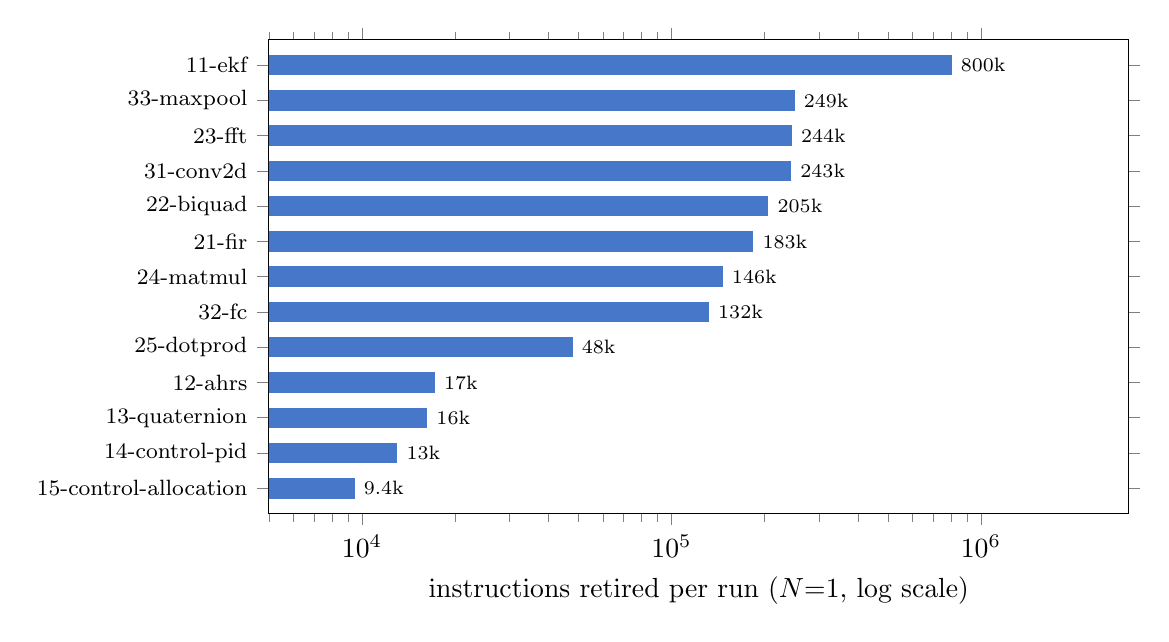
\begin{tikzpicture}
\begin{axis}[
  xbar, xmode=log, width=12.5cm, height=7.6cm,
  xlabel={instructions retired per run ($N{=}1$, log scale)},
  xmin=5000, xmax=3000000,
  bar width=7pt, enlarge y limits=0.06,
  symbolic y coords={15-control-allocation,14-control-pid,13-quaternion,12-ahrs,25-dotprod,32-fc,24-matmul,21-fir,22-biquad,31-conv2d,23-fft,33-maxpool,11-ekf},
  ytick=data, y tick label style={font=\footnotesize}, tick align=outside,
  nodes near coords, nodes near coords align={horizontal},
  nodes near coords style={font=\scriptsize, anchor=west}, point meta=explicit symbolic,
]
\addplot[fill=cArm,draw=cArm] coordinates {
 (9429,15-control-allocation)[9.4k] (12965,14-control-pid)[13k] (16185,13-quaternion)[16k]
 (17133,12-ahrs)[17k] (47737,25-dotprod)[48k] (131653,32-fc)[132k] (145892,24-matmul)[146k]
 (183221,21-fir)[183k] (204933,22-biquad)[205k] (242732,31-conv2d)[243k] (243947,23-fft)[244k]
 (249071,33-maxpool)[249k] (800482,11-ekf)[800k]};
\end{axis}
\end{tikzpicture}
\caption{Per-run AVR instruction count. Even ``cheap'' control kernels cost thousands of instructions
because every fp operation is a softfloat call.}\label{fig:insts}
\end{figure}

\paragraph{What they use most (EKF worked example).}
The per-mnemonic op-mix of the EKF predict is dominated by multi-byte integer add/subtract-with-carry,
branches, and shifts---i.e.\ software floating point on a core with no FPU:
\code{adc} 142\,234, \code{cpc} 68\,584, \code{brbs} 65\,976, \code{brbc} 59\,117, \code{add} 57\,168,
\code{eor} 37\,066, \code{ror} 34\,764, $\dots$ (53 distinct mnemonics totalling the 800\,482 instructions).
Attributing instructions to functions makes the cause explicit: \textbf{82.1\,\% of EKF cycles are spent
in compiler arithmetic-helper routines}. Decomposing the runtime cost as
$\text{cost}=\text{calls}\times\text{cycles/call}$ (Table~\ref{tab:cost}, Figure~\ref{fig:ekfcost}) shows
where the time goes and, crucially, the \emph{operation counts} a hardware datapath would replace.

\begin{table}[ht]\centering\small
\caption{EKF predict: runtime cost by function (one predict + startup).}\label{tab:cost}
\begin{tabular}{@{}lrrr@{}}
\toprule
function & cost (cycles) & calls & cycles/call \\
\midrule
\ds\ (fp divide) & 233\,106 & 552 & 422.3 \\
\code{main} (the kernel itself) & 147\,140 & 1 & 147\,140 \\
\ms\ (fp multiply) & 112\,826 & 1\,601 & 70.5 \\
\as\ (fp add) & 98\,802 & 1\,673 & 59.1 \\
\code{\_\_floatsisf} (int$\rightarrow$float) & 65\,111 & 1\,152 & 56.5 \\
\code{\_\_udivmodhi4} (integer divide, used by fp) & 53\,888 & 8\,832 & 6.1 \\
\bottomrule
\end{tabular}
\end{table}

\begin{figure}[ht]\centering
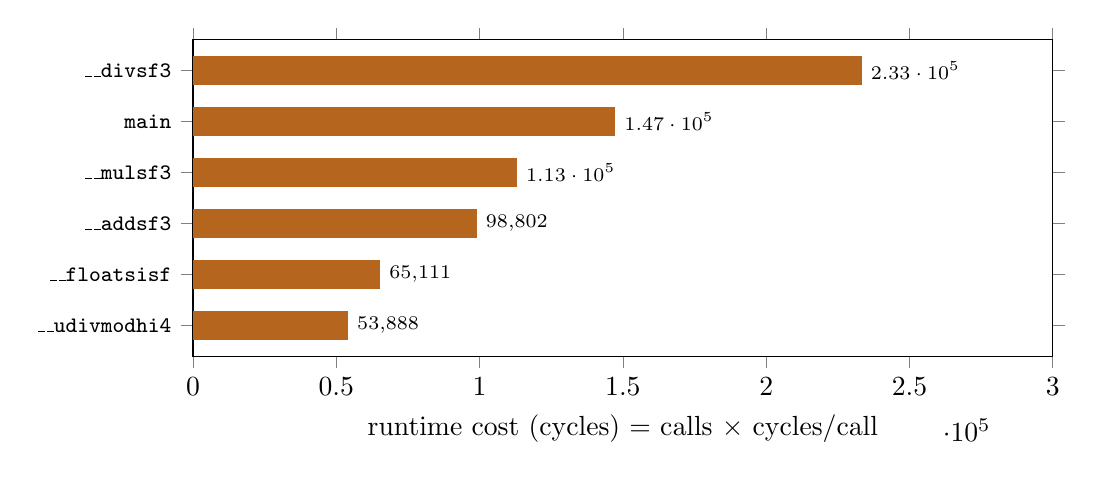
\begin{tikzpicture}
\begin{axis}[
  xbar, width=12.5cm, height=5.6cm,
  xlabel={runtime cost (cycles) $=$ calls $\times$ cycles/call},
  xmin=0, xmax=300000, bar width=10pt, enlarge y limits=0.12,
  ytick={0,1,2,3,4,5},
  yticklabels={\texttt{\_\_udivmodhi4},\texttt{\_\_floatsisf},\texttt{\_\_addsf3},\texttt{\_\_mulsf3},\texttt{main},\texttt{\_\_divsf3}},
  y tick label style={font=\footnotesize}, tick align=outside,
  nodes near coords, nodes near coords align={horizontal},
  nodes near coords style={font=\scriptsize, anchor=west},
]
\addplot[fill=cRv,draw=cRv] coordinates {(53888,0)(65111,1)(98802,2)(112826,3)(147140,4)(233106,5)};
\end{axis}
\end{tikzpicture}
\caption{Where EKF cycles go. Floating-point divide (\ds) is the single largest cost; the softfloat
helpers together are 82\,\% of all cycles.}\label{fig:ekfcost}
\end{figure}

\noindent Two observations generalize across the suite: \textbf{(a)} fp work is overwhelmingly softfloat,
and \textbf{(b)} the \emph{mix} of fp ops differs by kernel---the EKF is \emph{division}-heavy (552
divides at $\sim$422 cycles each, the single largest cost), whereas Madgwick AHRS, by design, uses a fast
inverse-square-root bit trick and issues \emph{zero} divisions and is multiply-bound. The int8 kernels
contain \emph{no} softfloat at all---their hot op is an integer multiply (\code{\_\_umulhisi3}). This
fp-divide / fp-multiply / int8-MAC split is the primary input to ISA design (\S6).

\section{(\S2) Roofline / Headroom Model}

To turn the characterization into a design verdict we plot each kernel on a roofline
(Figure~\ref{fig:roofline}). Per-invocation operation count (softfloat calls for fp kernels), bytes moved
(load/store count), and cycles are taken from the two-run difference. The model assumes AVR data-memory
bandwidth $\text{BW}=0.5$~byte/cycle (load/store $\approx$2 cycles/byte), a hardware-arithmetic compute
roof of $W$ ops/cycle at SIMD width $W$, and a memory$\leftrightarrow$compute ridge at intensity $I=2W$
ops/byte.

\begin{figure}[ht]\centering
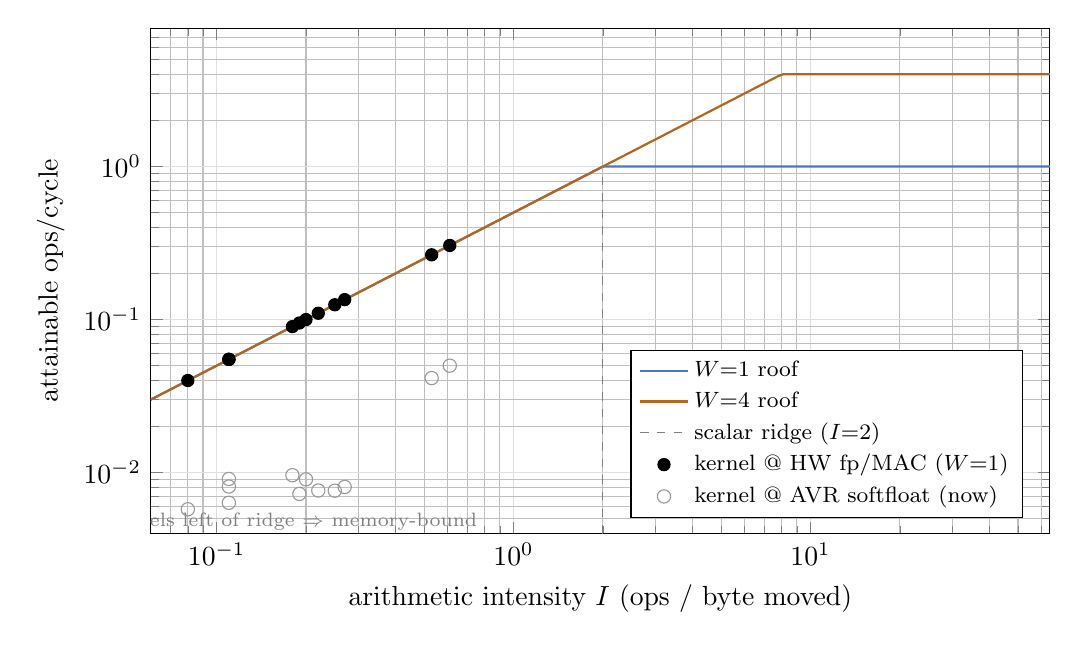
\begin{tikzpicture}
\begin{axis}[
  xmode=log, ymode=log, width=13cm, height=8cm,
  xlabel={arithmetic intensity $I$ (ops / byte moved)},
  ylabel={attainable ops/cycle},
  xmin=0.06, xmax=64, ymin=0.004, ymax=8,
  legend pos=south east, legend cell align=left, legend style={font=\footnotesize},
  grid=both, major grid style={line width=.2pt,draw=gray!25}, minor tick num=1,
]
% W=1 and W=4 hardware-arithmetic roofs (perf = min(W, BW*I))
\addplot[cArm,thick,domain=0.06:64,samples=200]{min(1,0.5*x)}; \addlegendentry{$W{=}1$ roof}
\addplot[cRv,thick,domain=0.06:64,samples=200]{min(4,0.5*x)};  \addlegendentry{$W{=}4$ roof}
% scalar ridge (W=1) at I=2
\addplot[gray,dashed] coordinates {(2,0.004)(2,1)};
\addlegendentry{scalar ridge ($I{=}2$)}
% kernels at HW-fp (W=1) attainable perf
\addplot[only marks,mark=*,mark size=2.2pt,black] coordinates {
 (0.27,0.135)(0.25,0.125)(0.22,0.11)(0.20,0.10)(0.19,0.095)(0.18,0.09)
 (0.11,0.055)(0.11,0.055)(0.11,0.055)(0.08,0.04)(0.61,0.305)(0.53,0.265)};
\addlegendentry{kernel @ HW fp/MAC ($W{=}1$)}
% kernels at softfloat baseline
\addplot[only marks,mark=o,mark size=2.4pt,cBase] coordinates {
 (0.27,0.00807)(0.25,0.00763)(0.22,0.00765)(0.20,0.00905)(0.19,0.00727)(0.18,0.00963)
 (0.11,0.00812)(0.11,0.0091)(0.11,0.00636)(0.08,0.00577)(0.61,0.05)(0.53,0.0415)};
\addlegendentry{kernel @ AVR softfloat (now)}
\node[font=\scriptsize,gray] at (axis cs:0.16,0.0048) {all kernels left of ridge $\Rightarrow$ memory-bound};
\end{axis}
\end{tikzpicture}
\caption{Roofline. Vertical gap between an open (softfloat, now) and filled (HW fp) marker is the
attainable speedup ($\approx$6--16$\times$). Every kernel sits \emph{left} of the scalar ridge, so the
filled markers ride the sloped (memory-bound) part of the roof---widening $W$ lifts the flat roof but not
these points: \textbf{wide SIMD is wasted}.}\label{fig:roofline}
\end{figure}

\begin{table}[ht]\centering\small
\caption{Roofline (per invocation, i11$-$i1). \emph{helper\%} $=$ cycles in arithmetic-helper routines;
\emph{sp@W} $=$ attainable speedup over softfloat with a HW datapath at SIMD width $W$.}\label{tab:roof}
\begin{tabular}{@{}llrrrrrrr@{}}
\toprule
workload & kind & ops & bytes & cyc/op & $I$ (op/B) & helper\% & ridge\,$W$ & sp@1 / @4 / @8 \\
\midrule
12-ahrs & fp & 181 & 680 & 123.9 & 0.27 & 98.2 & 0.1 & 16.5 / 16.5 / 16.5 \\
25-dotprod & fp & 131 & 528 & 131.1 & 0.25 & 83.8 & 0.1 & 16.3 / 16.3 / 16.3 \\
24-matmul & fp & 1034 & 4644 & 130.7 & 0.22 & 83.5 & 0.1 & 14.6 / 14.6 / 14.6 \\
11-ekf & fp & 2500 & 12788 & 110.5 & 0.20 & 97.8 & 0.1 & 10.8 / 10.8 / 10.8 \\
21-fir & fp & 1586 & 8254 & 137.5 & 0.19 & 79.0 & 0.1 & 13.2 / 13.2 / 13.2 \\
13-quaternion & fp & 145 & 806 & 103.9 & 0.18 & 85.0 & 0.1 & 9.3 / 9.3 / 9.3 \\
22-biquad & fp & 2162 & 19316 & 123.2 & 0.11 & 85.8 & 0.1 & 6.9 / 6.9 / 6.9 \\
23-fft & fp & 2754 & 25292 & 109.9 & 0.11 & 77.1 & 0.1 & 6.0 / 6.0 / 6.0 \\
15-control-alloc & fp & 36 & 332 & 157.3 & 0.11 & 77.5 & 0.1 & 8.5 / 8.5 / 8.5 \\
14-control-pid & fp & 51 & 603 & 173.4 & 0.08 & 90.9 & 0.0 & 7.3 / 7.3 / 7.3 \\
32-fc & int8 & 2048 & 3338 & 20.0 & 0.61 & 58.5 & 0.3 & 6.1 / 6.1 / 6.1 \\
31-conv2d & int8 & 10368 & 19738 & 24.1 & 0.53 & 59.1 & 0.3 & 6.3 / 6.3 / 6.3 \\
\bottomrule
\end{tabular}
\end{table}

\paragraph{Verdict.} Three conclusions follow, and they are nuanced:
\begin{enumerate}
  \item \textbf{The baseline is compute(softfloat)-bound.} 58--98\,\% of cycles are in arithmetic helpers
  at $\sim$100--170 cycles per fp op, so a scalar hardware fp/MAC datapath removes that tax for
  $\approx$\,\textbf{6--16$\times$} (the \emph{sp@1} column).
  \item \textbf{But arithmetic intensity is low} (0.08--0.61 ops/byte), far left of the scalar ridge
  ($I{=}2$). Hence once arithmetic is in hardware the kernels become \emph{memory-bound}: every
  $\text{ridge}\,W<1$, and \emph{sp@1 $=$ sp@4 $=$ sp@8}---\textbf{wide SIMD does not help}; the ceiling is
  memory bandwidth, not compute.
  \item \textbf{Design implication:} prioritize a hardware fp/MAC datapath \emph{plus} memory bandwidth
  (wider/multi-byte loads, a local scratchpad) over many vector lanes. The classic ``memory-bound kills
  SIMD'' kill-criterion \emph{does} bite---it kills wide SIMD, but \emph{not} the hardware-arithmetic
  datapath, which still delivers 6--16$\times$.
\end{enumerate}
\emph{Caveat:} \texttt{bytes} is the load/store count; for the big-expression EKF some are register spills,
so per-kernel intensity is approximate, but the order-of-magnitude ($I\ll$ ridge) result is robust across
all kernels. \code{33-maxpool} is excluded (no MAC---pure int8 compares).

\subsection{Where the FPU architectures sit: a measured cross-architecture roofline}\label{sec:xarch}
The roofline above is AVR-only. To see how much of the gap is the \emph{missing FPU} versus the
\emph{ISA encoding}, the same fp kernels were measured on ARM64 and RISC-V (\S3's runs) and placed on the
\emph{same} roofline (Figure~\ref{fig:xroof}, Table~\ref{tab:xarch}). Two quantities are taken
per-invocation (i11$-$i1) for each ISA: \textbf{achieved throughput} (fp-ops/cycle) and \textbf{arithmetic
intensity} (fp-ops per data-byte). To keep the byte axis architecture-neutral, \texttt{bytes} here is the
gem5 \emph{memory-controller} data traffic (\code{bytesRead/Written::cpu.data}, total data memory incl.\
stack spills) for all three ISAs; fp-ops are softfloat calls on AVR and committed float-class instructions
on ARM/RISC-V.

\begin{figure}[ht]\centering
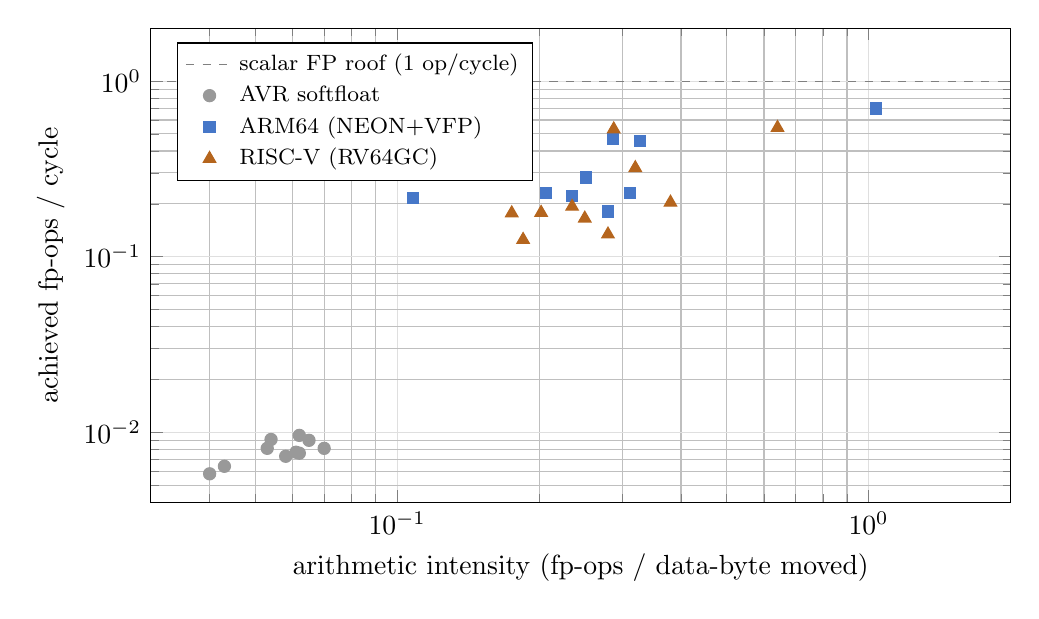
\begin{tikzpicture}
\begin{axis}[
  xmode=log, ymode=log, width=12.5cm, height=7.6cm,
  xlabel={arithmetic intensity (fp-ops / data-byte moved)},
  ylabel={achieved fp-ops / cycle},
  xmin=0.03, xmax=2, ymin=0.004, ymax=2,
  legend pos=north west, legend cell align=left, legend style={font=\footnotesize},
  grid=both, major grid style={line width=.2pt,draw=gray!25}, minor tick num=1,
]
\addplot[gray,dashed,domain=0.03:2,samples=2]{1}; \addlegendentry{scalar FP roof (1 op/cycle)}
\addplot[only marks,mark=*,mark size=2.2pt,cBase] coordinates {
 (0.070,0.0081)(0.062,0.0076)(0.061,0.0077)(0.065,0.0090)(0.058,0.0073)
 (0.062,0.0096)(0.053,0.0081)(0.054,0.0091)(0.043,0.0064)(0.040,0.0058)};
\addlegendentry{AVR softfloat}
\addplot[only marks,mark=square*,mark size=2pt,cArm] coordinates {
 (1.039,0.6985)(0.251,0.2824)(0.235,0.2223)(0.287,0.4703)(0.280,0.1808)
 (0.327,0.4552)(0.175,0.3185)(0.207,0.2310)(0.108,0.2156)(0.312,0.2307)};
\addlegendentry{ARM64 (NEON+VFP)}
\addplot[only marks,mark=triangle*,mark size=2.6pt,cRv] coordinates {
 (0.641,0.5424)(0.250,0.1652)(0.235,0.1929)(0.288,0.5322)(0.280,0.1341)
 (0.320,0.3201)(0.175,0.1770)(0.202,0.1781)(0.185,0.1249)(0.380,0.2036)};
\addlegendentry{RISC-V (RV64GC)}
\end{axis}
\end{tikzpicture}
\caption{The same ten fp kernels on three ISAs. AVR (grey) clusters at the bottom-left
($\sim$0.006--0.010 fp-ops/cycle); the FPU cores (blue/orange) sit two orders of magnitude higher, near
the scalar FP roof, \emph{and} further right (higher intensity)---softfloat both lacks hardware fp
\emph{and} moves $\sim$5$\times$ more bytes per op.}\label{fig:xroof}
\end{figure}

\begin{table}[ht]\centering\small
\caption{Cross-architecture arithmetic analysis (per invocation, i11$-$i1).
$I$ $=$ fp-ops/data-byte (intensity); \emph{tput} $=$ achieved fp-ops/cycle.}\label{tab:xarch}
\begin{tabular}{@{}lrrrrrrr@{}}
\toprule
& \multicolumn{2}{c}{AVR softfloat} & \multicolumn{2}{c}{ARM64} & \multicolumn{2}{c}{RISC-V} & ARM/AVR \\
\cmidrule(lr){2-3}\cmidrule(lr){4-5}\cmidrule(lr){6-7}
workload & $I$ & tput & $I$ & tput & $I$ & tput & tput \\
\midrule
12-ahrs & 0.070 & 0.0081 & 1.039 & 0.699 & 0.641 & 0.542 & 86.5$\times$ \\
25-dotprod & 0.062 & 0.0076 & 0.251 & 0.282 & 0.250 & 0.165 & 37.0$\times$ \\
24-matmul & 0.061 & 0.0077 & 0.235 & 0.222 & 0.235 & 0.193 & 29.1$\times$ \\
11-ekf & 0.065 & 0.0090 & 0.287 & 0.470 & 0.288 & 0.532 & 52.0$\times$ \\
21-fir & 0.058 & 0.0073 & 0.280 & 0.181 & 0.280 & 0.134 & 24.9$\times$ \\
13-quaternion & 0.062 & 0.0096 & 0.327 & 0.455 & 0.320 & 0.320 & 47.3$\times$ \\
22-biquad & 0.053 & 0.0081 & 0.175 & 0.319 & 0.175 & 0.177 & 39.2$\times$ \\
23-fft & 0.054 & 0.0091 & 0.207 & 0.231 & 0.202 & 0.178 & 25.4$\times$ \\
15-control-alloc & 0.043 & 0.0064 & 0.108 & 0.216 & 0.185 & 0.125 & 33.9$\times$ \\
14-control-pid & 0.040 & 0.0058 & 0.312 & 0.231 & 0.380 & 0.204 & 40.0$\times$ \\
\bottomrule
\end{tabular}
\end{table}

\noindent\textbf{What this adds to the verdict.}
\begin{itemize}
  \item \textbf{Throughput.} The FPU cores reach \textbf{0.13--0.70 fp-ops/cycle} (within a small factor of
  the scalar FP roof of 1), versus AVR softfloat's \textbf{0.006--0.010}---a \textbf{25--86$\times$} gap
  that tracks the \S3 instruction-count gap. This confirms the deficit is the \emph{absent hardware FPU},
  not the AVR instruction encoding, and bounds what a hardware fp datapath can recover.
  \item \textbf{Intensity.} AVR's measured intensity (0.04--0.07 fp/byte) is \textbf{$\sim$3--15$\times$
  lower} than ARM's (0.11--1.04): softfloat spills $\sim$5$\times$ more bytes per fp op, pushing AVR
  \emph{deeper} into the memory-bound region. So even after adding hardware fp, AVR-XPU must pair the MAC
  datapath with enough memory bandwidth to feed it---reinforcing the \S2 design implication.
  \item \emph{Caveat:} where gcc auto-vectorized for NEON (notably \code{21-fir}), one ARM instruction
  packs several fp ops, so ARM's fp-op count---and thus its intensity/throughput---is slightly
  \emph{under}-stated for those kernels.
\end{itemize}

\section{(\S3) Baseline Comparison: ARM and RISC-V with hardware FP}

To quantify what the AVR-XPU must beat, the \emph{same} C kernels were cross-compiled for AArch64
(NEON+VFP) and RV64GC (scalar F/D) and run on gem5's multi-ISA build. Because all three ISAs implement
IEEE-754, the host CRC validates AVR, ARM, \emph{and} RISC-V identically (the \texttt{crc} column).
Per-invocation instruction counts (i11$-$i1) are model-independent and directly comparable
(Figure~\ref{fig:speedup}); cycle counts are not (different CPU models), so we report instructions.

\begin{figure}[ht]\centering
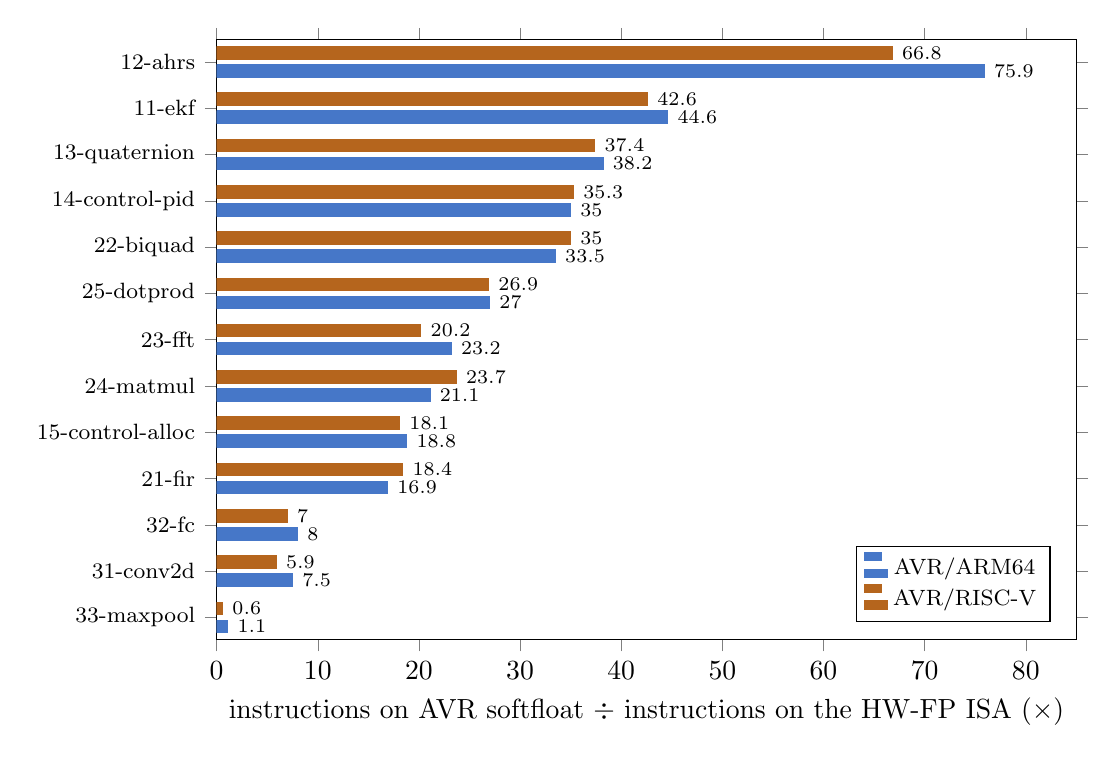
\begin{tikzpicture}
\begin{axis}[
  xbar, width=12.5cm, height=9.2cm,
  xlabel={instructions on AVR softfloat $\div$ instructions on the HW-FP ISA ($\times$)},
  xmin=0, xmax=85, bar width=4.5pt, enlarge y limits=0.04,
  symbolic y coords={33-maxpool,31-conv2d,32-fc,21-fir,15-control-alloc,24-matmul,23-fft,25-dotprod,22-biquad,14-control-pid,13-quaternion,11-ekf,12-ahrs},
  ytick=data, y tick label style={font=\footnotesize}, tick align=outside,
  legend pos=south east, legend style={font=\footnotesize},
  nodes near coords, nodes near coords style={font=\scriptsize,/pgf/number format/fixed,/pgf/number format/precision=1},
]
\addplot[fill=cArm,draw=cArm] coordinates {
 (1.1,33-maxpool)(7.5,31-conv2d)(8.0,32-fc)(16.9,21-fir)(18.8,15-control-alloc)(21.1,24-matmul)
 (23.2,23-fft)(27.0,25-dotprod)(33.5,22-biquad)(35.0,14-control-pid)(38.2,13-quaternion)(44.6,11-ekf)(75.9,12-ahrs)};
\addplot[fill=cRv,draw=cRv] coordinates {
 (0.6,33-maxpool)(5.9,31-conv2d)(7.0,32-fc)(18.4,21-fir)(18.1,15-control-alloc)(23.7,24-matmul)
 (20.2,23-fft)(26.9,25-dotprod)(35.0,22-biquad)(35.3,14-control-pid)(37.4,13-quaternion)(42.6,11-ekf)(66.8,12-ahrs)};
\legend{AVR/ARM64, AVR/RISC-V}
\end{axis}
\end{tikzpicture}
\caption{How many \emph{more} instructions AVR softfloat needs than an FPU-equipped core, per invocation.
fp kernels (top) cost 17--76$\times$; int8 kernels (bottom three) only 6--8$\times$; pure-compare
\code{maxpool} is a wash ($\sim$1$\times$, RISC-V worse).}\label{fig:speedup}
\end{figure}

\begin{table}[ht]\centering\small
\caption{AVR softfloat vs.\ ARM64 / RISC-V with hardware FP: instructions \emph{per invocation}.
\emph{fp(A/Ar/Rv)} $=$ fp ops issued on each (softfloat \emph{calls} for AVR; fp \emph{instructions} for
ARM/RISC-V). All CRC-validated.}\label{tab:base}
\begin{tabular}{@{}lrrrrrr@{}}
\toprule
workload & AVR insts & ARM insts & RV insts & AVR/ARM & AVR/RV & fp A/Ar/Rv \\
\midrule
12-ahrs & 16\,368 & 216 & 245 & \textbf{75.9$\times$} & 66.8$\times$ & 181/184/220 \\
11-ekf & 195\,970 & 4\,398 & 4\,600 & \textbf{44.6$\times$} & 42.6$\times$ & 2500/2161/3998 \\
13-quaternion & 10\,396 & 272 & 278 & 38.2$\times$ & 37.4$\times$ & 145/130/230 \\
14-control-pid & 6\,445 & 184 & 182 & 35.0$\times$ & 35.3$\times$ & 51/96/128 \\
22-biquad & 187\,133 & 5\,583 & 5\,340 & 33.5$\times$ & 35.0$\times$ & 2162/1970/4517 \\
25-dotprod & 12\,520 & 463 & 466 & 27.0$\times$ & 26.9$\times$ & 131/131/263 \\
23-fft & 210\,060 & 9\,045 & 10\,386 & 23.2$\times$ & 20.2$\times$ & 2754/2178/4805 \\
24-matmul & 97\,756 & 4\,643 & 4\,133 & 21.1$\times$ & 23.7$\times$ & 1034/1034/2197 \\
15-control-alloc & 4\,043 & 215 & 223 & 18.8$\times$ & 18.1$\times$ & 36/47/99 \\
21-fir & 159\,353 & 9\,423 & 8\,653 & 16.9$\times$ & 18.4$\times$ & 1586/2354/3821 \\
\midrule
32-fc & 26\,579 & 3\,308 & 3\,808 & 8.0$\times$ & 7.0$\times$ & 0/0/0 \\
31-conv2d & 172\,350 & 23\,003 & 29\,080 & 7.5$\times$ & 5.9$\times$ & 0/0/0 \\
33-maxpool & 5\,201 & 4\,878 & 8\,128 & 1.1$\times$ & 0.6$\times$ & 0/0/0 \\
\bottomrule
\end{tabular}
\end{table}

\paragraph{Findings.}
\begin{itemize}
  \item On the fp kernels, an FPU-equipped ARM needs \textbf{17--76$\times$ fewer instructions} than AVR
  softfloat (RISC-V similar, slightly less because gcc auto-vectorizes for NEON but not for scalar RV64).
  This is the FPU advantage stated plainly: AVR turns each fp op into a $\sim$50--170-instruction softfloat
  call; ARM/RISC-V do it in $\approx$1.
  \item The \textbf{int8 kernels show only 6--8$\times$} (all three issue integer MACs; AVR's penalty there
  is its 8-bit width, not softfloat), and \textbf{\code{maxpool} $\approx$1$\times$}---a pure-compare
  kernel where AVR is competitive and 64-bit RISC-V is actually \emph{worse} (0.6$\times$).
  \item \textbf{Implication.} AVR-XPU cannot beat an FPU-equipped ARM/RISC-V on raw fp instruction count.
  Per the plan, its case must therefore rest on \emph{energy/area} for a stripped, domain-specific
  datapath, not on throughput.
\end{itemize}

\section{Synthesis and Implications for ISA Design (\S4)}
The three gates compose into a coherent, data-backed steer:
\begin{itemize}
  \item \textbf{There is a real opportunity} (\S2: 6--16$\times$ from removing softfloat) but
  \textbf{a hard ceiling} (\S2: low intensity $\Rightarrow$ memory-bound $\Rightarrow$ wide SIMD wasted;
  \S3: an off-the-shelf FPU already captures 17--76$\times$).
  \item The defensible target is therefore a \textbf{minimal hardware fp/int8 MAC datapath fed by good
  memory bandwidth} (wide/multi-byte loads, local scratchpad), \textbf{not} a wide vector machine---and
  the competitive axis is \textbf{energy/area per operation}, not peak FLOPS.
  \item The op-mix prioritizes which primitives matter: a fused \textbf{fp multiply-add} and a
  \textbf{fp divide / reciprocal} (the EKF's single largest cost) for Cat-1/2, and a packed
  \textbf{int8 MAC + requantize} for Cat-3.
\end{itemize}

\section{Threats to Validity}
\begin{itemize}
  \item gem5's ARM/RISC-V models are application-class (A-profile with NEON), not Cortex-M; instruction
  counts are robust, but cycle/energy comparison needs real M-profile hardware---the planned next step
  (Cortex-M boards with the DWT cycle counter and current measurement).
  \item Cycle figures use each model's timing; cross-ISA cycle comparison is therefore avoided in favour
  of instruction counts. AVR cycle costs follow the instruction-set manual (validated against ATmega328P).
  \item Arithmetic intensity uses the softfloat-inclusive load/store count; the conclusion (intensity
  $\ll$ ridge) is order-of-magnitude robust but per-kernel values are approximate.
  \item Microkernels match the \emph{scalar} reference forms; vectorized library variants (Helium/MVE,
  RVV) would change ARM/RISC-V counts but not the qualitative gap. The primary M55+Helium baseline (\S3)
  remains to be added from cited/measured data.
\end{itemize}

\section*{Reproducibility}
All kernels, harness, instrumentation, per-run logs (op/cycle/function/call histograms, the runtime-cost
charts), and the analysis scripts (\code{roofline.py}, \code{compare\_isa.py}) are in
\href{https://github.com/ragnar-vallhala/AVR-XPU}{github.com/ragnar-vallhala/AVR-XPU} under
\code{feasibility/execution/}; the gem5 model is at
\href{https://github.com/ragnar-vallhala/gem5}{github.com/ragnar-vallhala/gem5} (branch \code{btp}).
Each run is recorded as a JSON record (schema \code{avrxpu-run/1}) indexed by \code{results/runs.csv}, with
the producing ELF archived by content hash. Build this report with \code{./build.sh} (runs \code{pdflatex}
twice so all cross-references resolve).

\end{document}
